\documentclass[11pt,a4paper]{article}
\usepackage[T1]{fontenc}
\usepackage[margin=2.3cm]{geometry}
\usepackage{amsmath,amssymb}
\usepackage{graphicx}
\usepackage[dvipsnames]{xcolor}
\usepackage{enumitem}
\usepackage[colorlinks=true,linkcolor=blue,urlcolor=blue]{hyperref}
\setlength{\parskip}{0.6em}
\setlength{\parindent}{0pt}
\begin{document}

\begin{center}{\LARGE\bfseries openqmintro}\\[0.4em]{\large Learn the basic ideas of quantum mechanics: superposition, measurement and tunnelling, in three sessions.}\\[0.2em]\small PAN IIT OSS explainer \textbullet{} secondary to diploma/undergrad (levels 3-5)\end{center}

\section*{Why this exists}
Quantum mechanics is the theory behind chemistry, lasers, semiconductors and the chips in a phone. This explainer shows the first ideas with three small models you can run: a photon that interferes with itself, an electron trapped in a box, and an electron that gets through a wall.

\section*{The end goal}
The end goal is to learn the basic ideas of quantum mechanics: superposition, measurement and tunnelling. The same ideas carry over to atoms, molecules, quantum dots and quantum computers, which use many more states and more careful models.

\section*{How the three sessions build up}
\begin{enumerate}[nosep]
\item \textbf{Session 1: Amplitudes and probabilities: a photon that is not a coin} (Level 1: conceptual interactive model, 60 min).
\item \textbf{Session 2: A particle in a box: energy levels, probability density and emitted light} (Level 2: mathematical engineering model, 75 min).
\item \textbf{Session 3: Tunnelling: getting through a wall, validated by a transfer matrix} (Level 3: simulation and validation, 90 min).
\end{enumerate}

\section{Session 1: Amplitudes and probabilities: a photon that is not a coin}

\subsection*{A. Real-world problem}
A single photon enters a beam splitter and can leave by one of two exits. If we put a second beam splitter after a small path-length difference, the photon leaves by the same exit every time for one setting and never for another. A coin that was flipped at the first splitter could never do that. What is the photon between the two splitters?

\subsection*{B. Concept and theory}
A two-state system has two possible results, called path 0 and path 1 (states |0> and |1>). Its state is a pair of numbers (a, b), the amplitudes. They can be complex numbers; for now think of them as real numbers that may be negative. The probabilities of finding the system in path 0 or 1 are P0 = |a|\textasciicircum{}2 and P1 = |b|\textasciicircum{}2, and they must add up to 1. A superposition is a state in which both a and b are not zero. A 50/50 beam splitter turns (a, b) into ((a + b), (a - b)) / sqrt(2). A phase shift multiplies the amplitude of path 1 by exp(i phi): its size is unchanged, but the amplitudes of the two paths now add or cancel differently at the next splitter. For a photon that enters path 0, the first splitter gives (1, 1) / sqrt(2), the phase gives (1, exp(i phi)) / sqrt(2), and the second splitter gives the exit 0 amplitude (1 + exp(i phi)) / 2, so P0 = cos\textasciicircum{}2(phi / 2) and P1 = sin\textasciicircum{}2(phi / 2). At phi = 0 the amplitudes add and the photon always leaves by exit 0; at phi = 180 degrees they cancel and it never does. A classical coin that is in path 0 or path 1 with probability 1/2 each would leave by either exit with probability 1/2 whatever the phase, because probabilities, unlike amplitudes, cannot cancel. The same 1/2 appears if a detector inside the interferometer finds out which path the photon took: the measurement turns the superposition into one definite path and the interference disappears.

\begin{itemize}[nosep]
\item a, b: amplitudes of path 0 and path 1 (numbers, possibly complex) (no unit)
\item P0, P1: probabilities |a|\textasciicircum{}2 and |b|\textasciicircum{}2 (no unit)
\item BS: 50/50 beam splitter, ((a + b), (a - b)) / sqrt(2) (no unit)
\item phi: phase shift on path 1, phi = 360 degrees x (path difference / wavelength) (degrees)
\item theta: preparation angle: the state (cos(theta/2), sin(theta/2)) (degrees)
\end{itemize}

\[ P_0 = |a|^{2},\qquad P_1 = |b|^{2},\qquad |a|^{2} + |b|^{2} = 1 \]

\[ \mathrm{BS}\begin{pmatrix} a\\ b\end{pmatrix} = \frac{1}{\sqrt 2}\begin{pmatrix} a + b\\ a - b\end{pmatrix} \]

\[ P_0 = \cos^{2}\frac{\varphi}{2},\qquad P_1 = \sin^{2}\frac{\varphi}{2}\qquad\left(\text{photon entering path 0}\right) \]

\subsection*{C. Visual explanation}
The first figure plots the probability of exit 0 against the phase shift. The solid curve is the photon: it swings between 1 and 0 and is exactly 1/2 at phi = 90 and 270 degrees. The dashed line is the classical coin, which stays at 1/2 for every phase. The second figure shows how the preparation angle theta sets the two probabilities of a state: P0 = cos\textasciicircum{}2(theta / 2) and P1 = sin\textasciicircum{}2(theta / 2), which always add up to 1.

\begin{figure}[h]\centering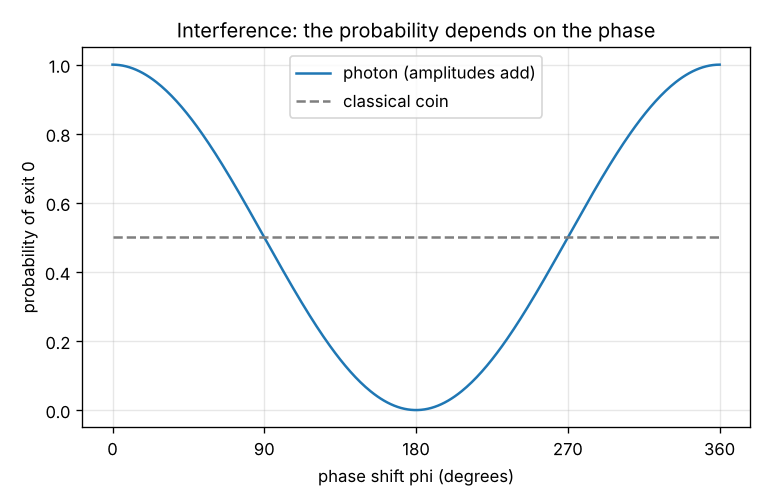
\includegraphics[width=0.78\textwidth]{figures/s01_interference.png}\caption{Probability of exit 0 against the phase shift: photon (solid) and classical coin (dashed).}\end{figure}

\begin{figure}[h]\centering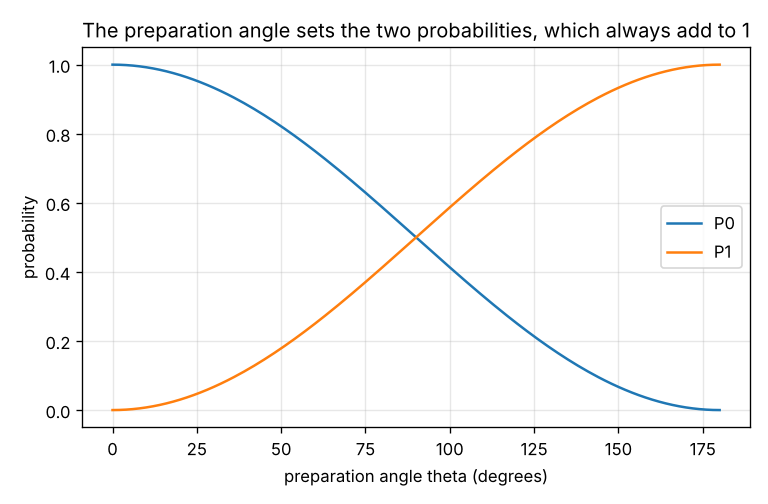
\includegraphics[width=0.78\textwidth]{figures/s01_preparation.png}\caption{The two probabilities of a state against its preparation angle.}\end{figure}

\subsection*{E. Worked example}
\textbf{Problem.} A photon enters path 0 of an interferometer with a phase shift of phi = 60 degrees on path 1. Find the amplitudes and the probability of each exit. Then do the same for a classical coin.

\begin{enumerate}[nosep]
\item First splitter: (1, 0) becomes (1, 1) / sqrt(2) = (0.707, 0.707): each path has probability 0.5.
\item Phase: path 1 is multiplied by exp(i 60 degrees) = 0.5 + 0.866i, giving (0.707, 0.354 + 0.612i).
\item Second splitter, exit 0: (0.707 + 0.354 + 0.612i) / sqrt(2) = 0.75 + 0.433i, so P0 = 0.75\textasciicircum{}2 + 0.433\textasciicircum{}2 = 0.75.
\item Exit 1: (0.707 - 0.354 - 0.612i) / sqrt(2) = 0.25 -0.433i, so P1 = 0.25. Check: 0.75 + 0.25 = 1.
\item Check with the formula: cos\textasciicircum{}2(30 degrees) = 0.75 and sin\textasciicircum{}2(30 degrees) = 0.25.
\item Coin: 0.5 and 0.5, whatever the phase.
\end{enumerate}
\textbf{Answer.} The photon leaves by exit 0 with probability 0.75 and by exit 1 with probability 0.25; a classical coin gives 0.5 and 0.5.

\section{Session 2: A particle in a box: energy levels, probability density and emitted light}

\subsection*{A. Real-world problem}
An electron is trapped in a very thin layer of semiconductor, about a nanometre wide. It can only take certain energies, and when it drops from one to a lower one it emits a photon of a definite colour. Which energies are allowed, where is the electron likely to be found, and what colour does it emit? This is the idea behind the quantum dots used in some displays.

\subsection*{B. Concept and theory}
A particle with momentum p behaves like a wave with wavelength lambda = h / p (de Broglie), where h = 6.626e-34 J s is the Planck constant. In a box of width L with impenetrable walls, the wave must be zero at both walls, so a whole number n of half-wavelengths must fit: lambda\_n = 2 L / n. The energy is E = p\textasciicircum{}2 / (2 m) = h\textasciicircum{}2 / (2 m lambda\textasciicircum{}2), which gives E\_n = n\textasciicircum{}2 h\textasciicircum{}2 / (8 m L\textasciicircum{}2) with n = 1, 2, 3 and so on. Only these energies are allowed; the lowest one, E\_1, is not zero because a wave that must fit in the box always has a wavelength of at most 2 L, so the particle can never be at rest. The wave function is psi\_n(x) = sqrt(2 / L) sin(n pi x / L) and the probability density is its square: the probability of finding the particle between x1 and x2 is the integral of the density, P = (x2 - x1) / L - [sin(2 n pi x2 / L) - sin(2 n pi x1 / L)] / (2 n pi). The density is zero at the nodes, so higher levels have more places where the particle is never found. When the particle drops from level k to level n, the energy difference leaves as a photon with wavelength lambda = h c / (E\_k - E\_n), about 1239.84 nm / (energy in eV).

\begin{itemize}[nosep]
\item n: level number (a whole number from 1) (no unit)
\item L: box width (nm)
\item m: particle mass (electron: 9.109e-31 kg) (kg)
\item h: Planck constant (J s (6.626e-34))
\item E\_n: energy of level n (eV (1 eV = 1.602e-19 J))
\item psi\_n, |psi\_n|\textasciicircum{}2: wave function and probability density (1/sqrt(nm), 1/nm)
\item u: relative position x / L (no unit)
\item lambda: wavelength of the emitted photon (nm)
\end{itemize}

\[ \lambda_n = \frac{2L}{n},\qquad E_n = \frac{n^{2} h^{2}}{8 m L^{2}} \]

\[ \psi_n(x) = \sqrt{\frac{2}{L}}\,\sin\frac{n\pi x}{L},\qquad P(x_1,x_2) = \frac{x_2 - x_1}{L} - \frac{\sin(2n\pi x_2/L) - \sin(2n\pi x_1/L)}{2n\pi} \]

\[ \lambda_{k\to n} = \frac{h c}{E_k - E_n}\approx \frac{1239.84\ \mathrm{nm\,eV}}{E_k - E_n} \]

\subsection*{C. Visual explanation}
The first figure plots the probability density times L for the levels n = 1, 2 and 3 against the relative position. Level 1 has one hump in the middle, level 2 has two humps and a node at the centre, level 3 has three humps. A classical particle would have a flat density (a value of 1 on this scale). The second figure plots the energy of the first three levels against the box width: every level rises as 1 / L\textasciicircum{}2 when the box is made narrower, and the gaps between them grow.

\begin{figure}[h]\centering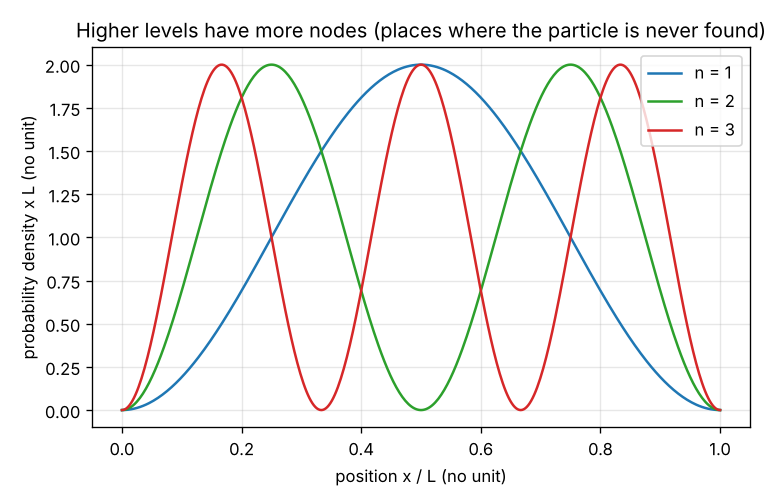
\includegraphics[width=0.78\textwidth]{figures/s02_density.png}\caption{Probability density (times L) of the first three levels against the relative position x / L.}\end{figure}

\begin{figure}[h]\centering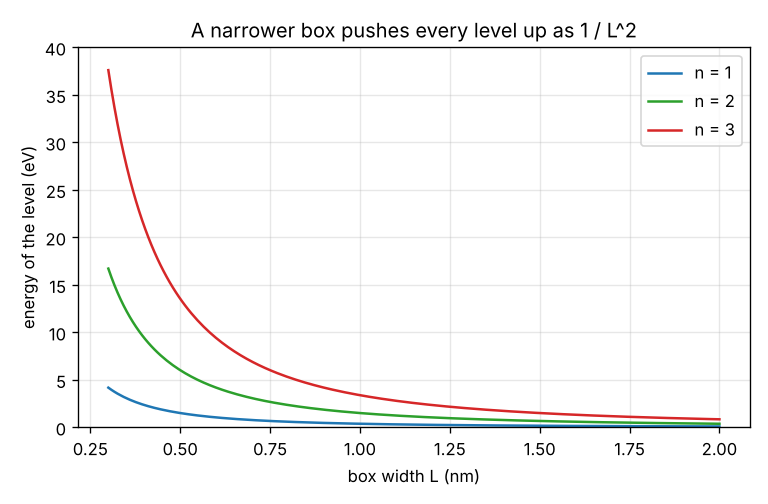
\includegraphics[width=0.78\textwidth]{figures/s02_levels_vs_width.png}\caption{Energy of the levels n = 1, 2 and 3 against the box width.}\end{figure}

\subsection*{E. Worked example}
\textbf{Problem.} An electron is in a box of width L = 1 nm. Find the energies of the first three levels, the wavelength of the photon emitted in the jump from level 2 to level 1, and the probability of finding the electron in the middle third of the box in levels 1 and 2.

\begin{enumerate}[nosep]
\item The constant is h\textasciicircum{}2 / (8 m L\textasciicircum{}2) = (6.626e-34)\textasciicircum{}2 / (8 x 9.109e-31 x (1e-9)\textasciicircum{}2) = 6.025e-20 J = 0.376 eV.
\item E\_1 = 0.376 eV, E\_2 = 4 x 0.376 = 1.504 eV and E\_3 = 9 x 0.376 = 3.384 eV.
\item The jump 2 to 1 releases 1.504 - 0.376 = 1.128 eV, so lambda = 1239.84 / 1.128 = 1099 nm. This is infrared, not visible.
\item Level 1, middle third (u from 1/3 to 2/3): P = 1/3 - [sin(4 pi / 3) - sin(2 pi / 3)] / (2 pi) = 0.609.
\item Level 2: P = 1/3 - [sin(8 pi / 3) - sin(4 pi / 3)] / (4 pi) = 0.196.
\item A classical particle would have 1/3 = 0.333: level 1 is more likely to be in the middle and level 2 much less likely.
\end{enumerate}
\textbf{Answer.} E\_1 = 0.376 eV, E\_2 = 1.504 eV, E\_3 = 3.384 eV; the 2 to 1 photon has 1099 nm (infrared); the middle third has probability 0.609 in level 1 and 0.196 in level 2.

\section{Session 3: Tunnelling: getting through a wall, validated by a transfer matrix}

\subsection*{A. Real-world problem}
A scanning tunnelling microscope (STM) holds a sharp metal tip a fraction of a nanometre above a surface. Electrons cross the empty gap even though they do not have the energy to climb out of the metal, and the current changes enormously when the tip moves by less than one atom. How large is the probability of getting through, how does it depend on the width of the gap, and can we trust a formula by checking it against a numerical solution?

\subsection*{B. Concept and theory}
An electron with energy E meets a barrier of height V0 and width a. Inside a region with potential V, the wave function satisfies hbar\textasciicircum{}2 / (2m) psi'' = (V - E) psi. Where E is above V the solutions oscillate with wave number k = sqrt((E - V) / (hbar\textasciicircum{}2 / 2m)); where E is below V, as inside a barrier, they grow or decay as exp(+/- kappa x) with kappa = sqrt((V0 - E) / (hbar\textasciicircum{}2 / 2m)). The constant hbar\textasciicircum{}2 / (2m) is 0.0381 eV nm\textasciicircum{}2 for an electron. The electron does not 'have' negative kinetic energy inside the barrier: only the amplitude of the wave reaches into it, and a little of it comes out on the other side. Matching the wave and its slope at both edges gives the exact transmission probability T = 1 / (1 + V0\textasciicircum{}2 sinh\textasciicircum{}2(kappa a) / (4 E (V0 - E))). For a thick barrier (kappa a above about 1) this is close to T = 16 E (V0 - E) / V0\textasciicircum{}2 x exp(-2 kappa a): the probability falls exponentially with the width, which is why tunnelling is so sensitive to small distances. For E above V0 the sinh becomes a sine, and T = 1 whenever a whole number of half-wavelengths fit in the barrier. As an independent check we cut a barrier into thin flat slices, match the wave and its slope at every interface and multiply the 2 x 2 matrices; for a single slice this must reproduce the exact formula and for a smooth barrier it gives the answer the formula cannot. The WKB estimate exp(-2 times the integral of kappa dx) is a third, quick check that works for thick smooth barriers.

\begin{itemize}[nosep]
\item E: energy of the electron (eV)
\item V0: height of the barrier (eV)
\item a: width of the barrier (nm)
\item kappa: decay constant inside the barrier, sqrt((V0 - E) / (hbar\textasciicircum{}2/2m)) (1/nm)
\item k: wave number where E is above the potential (1/nm)
\item T: transmission probability (no unit)
\item hbar\textasciicircum{}2/2m: 0.03810 for an electron (eV nm\textasciicircum{}2)
\item phi: work function (barrier height seen from the top of the metal) (eV)
\end{itemize}

\[ \kappa = \sqrt{\frac{V_0 - E}{\hbar^{2}/2m}},\qquad T = \frac{1}{1 + \dfrac{V_0^{2}\sinh^{2}(\kappa a)}{4E(V_0 - E)}} \]

\[ T \approx \frac{16E(V_0 - E)}{V_0^{2}}\,e^{-2\kappa a}\qquad(\kappa a \gtrsim 1) \]

\[ T_{\mathrm{WKB}} = \exp\!\left(-2\int_0^{a}\kappa(x)\,dx\right),\qquad \frac{I(d+\delta)}{I(d)} = e^{-2\kappa\delta} \]

\subsection*{C. Visual explanation}
The first figure plots the transmission against the width on a logarithmic scale for E = 1 eV and V0 = 2 eV: the exact curve is almost a straight line (an exponential), and the dashed thick-barrier approximation lies close to it once the barrier is wider than about 0.2 nm. The second figure plots the transmission against the electron energy for a 0.5 nm barrier of height 2 eV: the exact formula and the transfer matrix lie on top of each other, T rises steadily towards the barrier height and, above it, oscillates because waves reflected from the two edges interfere.

\begin{figure}[h]\centering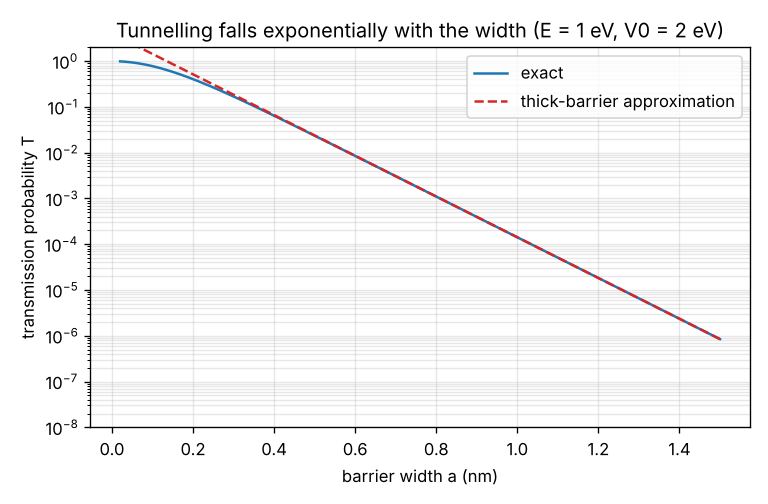
\includegraphics[width=0.78\textwidth]{figures/s03_transmission_vs_width.png}\caption{Transmission against barrier width on a logarithmic scale: exact formula and thick-barrier approximation.}\end{figure}

\begin{figure}[h]\centering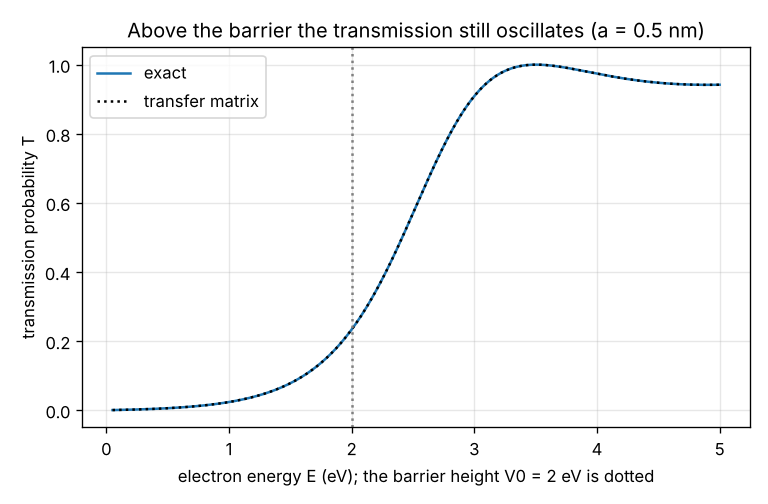
\includegraphics[width=0.78\textwidth]{figures/s03_transmission_vs_energy.png}\caption{Transmission against electron energy for a 0.5 nm barrier of 2 eV: exact formula and transfer matrix.}\end{figure}

\subsection*{E. Worked example}
\textbf{Problem.} An electron with E = 1 eV meets a barrier of height V0 = 2 eV and width a = 0.5 nm. Find kappa, the exact transmission, the thick-barrier estimate, and the factor by which an STM current changes when the tip is pulled back by 0.1 nm (work function 4.5 eV).

\begin{enumerate}[nosep]
\item kappa = sqrt((2 - 1) / 0.0381) = 5.123 per nm, so kappa a = 2.562.
\item sinh(2.562) = 6.440, so sinh\textasciicircum{}2 = 41.47.
\item T = 1 / (1 + 4 x 41.47 / (4 x 1 x 1)) = 1 / (1 + 41.47) = 0.0235: about 1 electron in 42 gets through.
\item Thick-barrier formula: 16 x 1 x 1 / 4 x exp(-2 x 2.562) = 4 x 0.00596 = 0.0238, within 1.2 percent of the exact value.
\item Check with the transfer matrix of one flat slice: it gives the same number (the checkpoint tests this for 75 cases).
\item STM: kappa = sqrt(4.5 / 0.0381) = 10.87 per nm, so pulling the tip back by 0.1 nm multiplies the current by exp(-2 x 10.87 x 0.1) = 0.114, that is the current falls to 1 in 8.8.
\end{enumerate}
\textbf{Answer.} kappa = 5.12 per nm; T = 0.0235 exactly and 0.0238 from the thick-barrier formula; the STM current falls by a factor 8.8 when the tip retracts by 0.1 nm.

\section*{Where to go next}
\begin{enumerate}[nosep]
\item \textbf{From the infinite box to the finite well.} Solve for the bound-state energies of a square well of finite depth by finding the roots of the matching conditions (or by a numerical eigenvalue solver).
\item \textbf{A wave packet in time.} A split-step or Crank-Nicolson solver that sends a Gaussian wave packet at a barrier and records the reflected and transmitted probabilities.
\item \textbf{The harmonic oscillator and molecular vibrations.} Numerical energy levels for the potential V = 1/2 k x\textasciicircum{}2 and the wavelength of the photon emitted in a jump between neighbouring levels for a diatomic molecule.
\item \textbf{The hydrogen atom.} A numerical solution of the radial equation and the wavelengths of the Balmer lines.
\item \textbf{Spin measurements in different directions.} Extend the two-state model of Session 1 to sequences of spin measurements along chosen angles, with the probabilities of each outcome.
\end{enumerate}

This is a simplified educational model. It is not a validated design tool and must not be used for real structures, electrical installations, vehicles, industrial processes or medical decisions.

\end{document}
